\documentclass[11pt, oneside]{article}   	% use "amsart" instead of "article" for AMSLaTeX format
\usepackage{geometry}                		% See geometry.pdf to learn the layout options. There are lots.
\geometry{a4paper}                   		% ... or a4paper or a5paper or letterpaper 
%\geometry{landscape}                		% Activate for rotated page geometry
\usepackage[parfill]{parskip}    			% Activate to begin paragraphs with an empty line rather than an indent
\usepackage{graphicx}				% Use pdf, png, jpg, or eps§ with pdflatex; use eps in DVI mode
								% TeX will automatically convert eps --> pdf in pdflatex		
\usepackage{amssymb}
\usepackage{amsmath}
\usepackage{algorithm}
\usepackage[noend]{algpseudocode}
\usepackage{float}
\usepackage{graphicx}
\graphicspath{ {/Users/yiqi/Desktop/School/Courses/ComsW4995_Design_Using_C++/Homeworks/hmwk3_c++/graphs/} }


%SetFonts

\title{Homework 3: Vector vs. List}
\author{Yi Qi, UNI: yq2211}
\date{2/5/2017}							% Activate to display a given date or no date

\begin{document}
\maketitle

$\bullet$ The initial random sequence is generated by calling \textbf{std::shuffle()} on a std::vector\(<\)int\(>\) of specified size \(n\). For fair comparison, the random deletion sequence is also generated beforehand.

$\bullet$ To construct both std::vector and std::list data, traverse the initial random vector and linear-search for the insertion point in the target container for each integer, then call the \textbf{std::insert()} function of the container to insert.

$\bullet$ To delete elements one at a time from the std::vector and the std::list, traverse the pre-generated deletion sequence and call the \textbf{std::erase()} function on each index.

$\bullet$ The \textbf{std::set} data structure is used for comparison. No algorithm is needed for insertion as the nature of std::set is to form an ordered sequence of keys, which are the unique integers from the initial sequence. For deletion it uses the same approach as others.

$\bullet$ To access a specific index in the container, first initialize an iterator variable to \textbf{std::begin}, then use the \textbf{std::move\_iterator::operator}\(\mathbf{++}\) in a for loop instead of calling the std::advance() or std::next() functions.


\section*{Results}

The execution time of insertion and deletion operations are illustrated below. 

\begin{figure}[H]
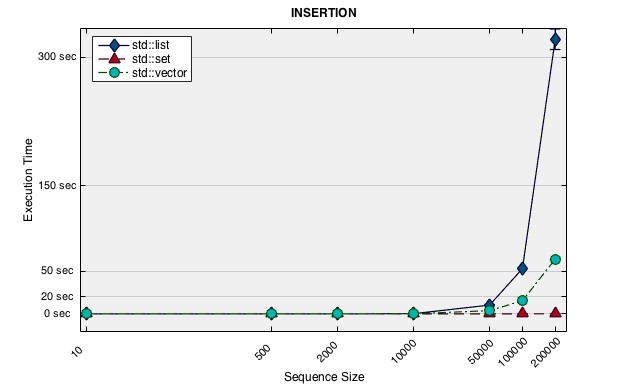
\includegraphics[width=\linewidth]{plot_insertion.png}
\caption{Execution Time of Insertion vs. Size of Input}
\end{figure}

\begin{figure}[H]
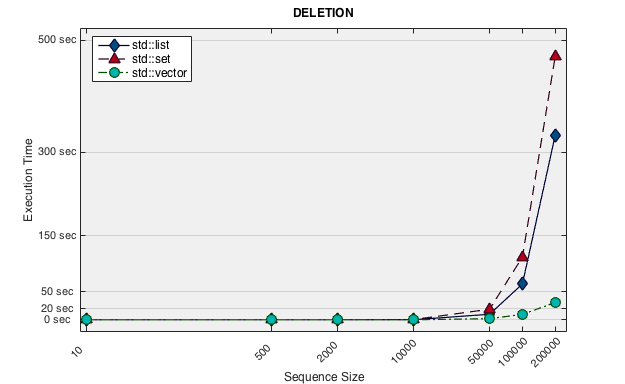
\includegraphics[width=\linewidth]{plot_deletion.png}
\caption{Execution Time of Deletion vs. Size of Input}
\end{figure}

$\bullet$ \textbf{std::vector}\\
Both insertion and deletion operations are fast, in almost linear time, although in theory it should of \(O(n^2)\) time. Although inserting and deleting an element involves shifting an expected 50\% members in the container, the elements are stored as an array in memory, which makes it much easier to copy them with caches.

$\bullet$ \textbf{std::list}\\
Both insertion and deletion operations perform with \(O(n^2)\) time as expected. Inserting and deleting element at any given index cost constant time for std::list, however traversing to that index takes much more time than traversing in std::vector, because of the scattered storage of std::list members in memory.

$\bullet$ \textbf{std::set}\\
The std::set is the perfect choice for the insertion operation, which almost takes constant time. The deletion, on the other hand, is the slowest because the deletion is by iterator. The std::set is simply not designed for such usage. It could be equally fast as insertion if erasing elements by their keys.

\section*{Experiments}

$\bullet$ Preallocation undermines the performance of insertion for both std::vector and std::list. Dynamic allocation has been made very efficient for these containers and should be adopted instead of preallocation.

$\bullet$ For std::vector the insertion time can be further improved with binary-search, while for std::list linear-search is faster due to less traversing. Using std::find\_if() with function object or Lambda expression does not improve the performance of insertion, probably because of the overhead of function calls.

$\bullet$ Using std::advance() improves the deletion performance of std::vector significantly, however it is not the case for std::list and std::set.

\end{document}  






